\documentclass[11pt]{article}
\usepackage[margin=1in]{geometry}
\usepackage{amsmath,amssymb}
\usepackage{booktabs}
\usepackage{array}
\usepackage{graphicx}
\usepackage{caption}
\usepackage{hyperref}

\newcommand{\dd}{\mathrm{d}}
\newcommand{\reD}{r_{eD}}
\newcommand{\pb}{\bar p}

\title{Pressure Build-up Tests in Heterogeneous Radial Reservoirs\\
\large Theory, a synthetic dataset, and a neural inverse model}
\date{\today}

\begin{document}
\maketitle

\begin{abstract}
A pressure build-up test shuts in a producing well and records how the bottomhole pressure recovers. Its purpose is
an inverse calculation: from one pressure curve, infer the permeability around the well, the skin, the wellbore
storage and the distance to the reservoir boundary. This report first develops the theory of build-up testing
(flow regimes, superposition, the Horner and derivative methods, and material balance with its dependence on the
initial pressure $p_i$), and then describes a set of numerical experiments: a validated finite-volume simulator,
a dataset of 20\,000 heterogeneous closed reservoirs, a check of what a build-up actually measures, a model-based
inversion, and a neural inverse model (a Fourier neural operator along log time) that returns the radial
permeability profile, the storage and the boundary distance with calibrated uncertainties. With the initial
pressure known and a precise gauge, the model recovers the boundary distance to 1--2\,\%; without $p_i$ the error
is about 20\,\%, for a physical reason discussed in Section~\ref{sec:mb}.
\end{abstract}

\tableofcontents

%======================================================================
\section{Introduction: what a build-up test is for}

A \emph{pressure transient test} perturbs a well's rate and records the bottomhole pressure response. Because the
pressure disturbance travels into the reservoir by diffusion, the response at early times reflects the well and
its immediate surroundings, and the response at later times reflects regions progressively farther away. Reading
the response as a function of time is therefore reading the reservoir as a function of distance.

Two elementary tests exist. In a \emph{drawdown} the well is opened and produced at (ideally) constant rate while
the flowing pressure $p_{wf}(t)$ falls. In a \emph{build-up} a well that has produced for a time $t_p$ is shut in
and the shut-in pressure $p_{ws}(\Delta t)$ recovers towards the reservoir pressure. Build-ups are the more common
diagnostic test in practice: a zero rate is exactly controlled (a constant nonzero rate rarely is), and the well is
tested without the rate fluctuations and gauge disturbances of flowing conditions. The price is lost production
during the shut-in, which limits how long a test can last.

A build-up interpretation delivers:
\begin{itemize}
  \item the \emph{permeability--thickness} $kh$ of the formation, from the radial-flow regime;
  \item the \emph{skin} $S$, the extra pressure drop near the well (damage or stimulation);
  \item the \emph{wellbore storage} $C$, the compressibility of the fluid column in the well;
  \item \emph{boundaries}: faults, the closed outer limit of the drainage area and its distance;
  \item the \emph{average reservoir pressure} $\pb$, needed for material balance and reserves.
\end{itemize}
The classical workflow identifies flow regimes on a log--log diagnostic plot (pressure change and its logarithmic
derivative), reads parameters from specialized plots (Horner, semilog, Cartesian), and refines them by matching an
analytical or numerical model to the data. The rest of the report builds this theory
(Section~\ref{sec:theory}) and then applies it to synthetic tests in heterogeneous reservoirs, where the classical
assumptions are strained (Sections~\ref{sec:data}--\ref{sec:nn}).

%======================================================================
\section{Theory of build-up testing}
\label{sec:theory}

\subsection{The radial diffusivity equation}

For single-phase flow of a slightly compressible fluid (constant viscosity $\mu$ and total compressibility $c_t$)
towards a vertical well of radius $r_w$ in a horizontal layer of thickness $h$ and porosity $\phi$, mass
conservation and Darcy's law give, for a permeability that varies with radius only,
\begin{equation}
  \phi \mu c_t \frac{\partial p}{\partial t} = \frac{1}{r}\frac{\partial}{\partial r}\!\left(r\,k(r)\,
  \frac{\partial p}{\partial r}\right), \qquad r_w \le r \le r_e .
  \label{eq:diffusivity}
\end{equation}
With a reference permeability $k_{\rm ref}$ and a reference rate $q$, the dimensionless variables
\begin{equation}
  r_D = \frac{r}{r_w},\quad
  t_D = \frac{k_{\rm ref}\, t}{\phi\mu c_t r_w^2},\quad
  k_D = \frac{k}{k_{\rm ref}},\quad
  p_D = \frac{2\pi k_{\rm ref} h\,(p_i - p)}{q B \mu},\quad
  C_D = \frac{C}{2\pi \phi c_t h r_w^2}
  \label{eq:dimless}
\end{equation}
($B$ is the formation volume factor, $C$ the wellbore storage coefficient) turn \eqref{eq:diffusivity} into
\begin{equation}
  \frac{\partial p_D}{\partial t_D} = \frac{1}{r_D}\frac{\partial}{\partial r_D}\!\left(r_D\,k_D\,
  \frac{\partial p_D}{\partial r_D}\right), \qquad 1 \le r_D \le \reD .
  \label{eq:diffD}
\end{equation}
$p_D$ is the pressure \emph{drop} below the initial pressure $p_i$, per unit rate: it starts at zero and grows as
the well produces. Time scales with $k/(\phi\mu c_t)$, the hydraulic diffusivity; for example, with
$k = 100$\,md, $\phi = 0.2$, $\mu = 1$\,cP, $c_t = 10^{-9}$\,Pa$^{-1}$ and $r_w = 0.1$\,m, one unit of $t_D$ is
0.02\,s, so $t_D = 10^6$ is about 5.6 hours.

\subsection{Boundary conditions: rate, storage, skin, closed boundary}

\paragraph{Well.} The well produces at a prescribed surface rate $q_D(t_D)$ (1 while producing, 0 after
shut-in). The fluid in the wellbore is compressible, so right after a rate change the sandface rate
$q_{sf}$ differs from the surface rate; the difference is the \emph{wellbore storage},
\begin{equation}
  C_D \frac{\dd p_{wD}}{\dd t_D} + q_{sfD} = q_D(t_D), \qquad
  q_{sfD} = -\left. k_D\, r_D \frac{\partial p_D}{\partial r_D}\right|_{r_D=1} .
  \label{eq:storage}
\end{equation}
\paragraph{Skin.} Drilling damage, perforations or stimulation change the permeability close to the well. The
classical \emph{thin skin} adds a pressure drop proportional to the sandface rate,
$p_{wD} = p_D(1) + S\, q_{sfD}$. A \emph{finite} altered zone of permeability $k_s$ out to $r_s$ in a formation of
permeability $k$ is equivalent in steady state to the skin of Hawkins,
\begin{equation}
  S = \left(\frac{k}{k_s} - 1\right)\ln\frac{r_s}{r_w},
  \label{eq:hawkins}
\end{equation}
positive for damage ($k_s<k$) and negative for stimulation.
\paragraph{Outer boundary.} A closed (no-flow) circular boundary at $r_e$: $\partial p_D/\partial r_D = 0$ at
$r_D = \reD$. The initial condition is $p_D = 0$ everywhere.

\subsection{Flow regimes of a drawdown}

For a homogeneous reservoir ($k_D = 1$) producing at unit rate, the well pressure goes through three regimes.

\paragraph{Wellbore storage.} At first the well produces fluid from the wellbore itself, so $q_{sfD}\approx 0$ and
\eqref{eq:storage} gives $p_{wD} = t_D / C_D$: a straight line of \emph{unit slope} on a log--log plot. Storage
effects fade after about $t_D \approx (60 + 3.5\,S)\,C_D$ (Ramey's rule of thumb).

\paragraph{Infinite-acting radial flow.} Before the boundary is felt, the reservoir behaves as if infinite. The
line-source solution $p_{wD} = \tfrac12 E_1\!\left(1/(4t_D)\right)$ becomes, for $t_D \gtrsim 25$,
\begin{equation}
  p_{wD} = \tfrac12\left(\ln t_D + 0.80907\right) + S ,
  \label{eq:semilog}
\end{equation}
a straight line in $\ln t$ of slope $1/2$ (for permeability $k$: slope $1/(2k_D)$ and $\ln(k_D t_D)$). In field
units this is the familiar semilog slope $m = 162.6\,qB\mu/(kh)$ psi per log cycle. The pressure front has then
reached roughly the \emph{radius of investigation} $r_{\rm inv,D} \approx 2\sqrt{k_D t_D}$, so the slope at time
$t$ reflects the permeability around that radius.

\paragraph{Pseudo-steady state.} Once the whole closed reservoir is drained, the pressure drops at the same rate
everywhere, and
\begin{equation}
  p_{wD} = \frac{2 t_D}{\reD^2 - 1} + \ln \reD - \frac34 + S .
  \label{eq:pss}
\end{equation}
The rate of decline $\dd p_{wD}/\dd t_D = 2/(\reD^2-1)$ is set by the pore volume alone; this is the basis of the
\emph{reservoir limit test}. The boundary starts to be felt around $t_D \approx \reD^2/(4 k_D)$.

\subsection{Superposition and the build-up}

Equation \eqref{eq:diffD} and its boundary conditions are linear in $p_D$, for any $k_D(r)$ and constant $C_D$,
$S$. A shut-in at $t_p$ is therefore the sum of the original production continued forever and an injection of the
same rate starting at $t_p$. With $p_{dd}(t)$ the unit-rate drawdown,
\begin{equation}
  p_{wD}(t_p + \Delta t) = p_{dd}(t_p + \Delta t) - p_{dd}(\Delta t), \qquad
  \Delta p_{bu}(\Delta t) = p_{ws} - p_{wf} = p_{dd}(t_p) - p_{dd}(t_p + \Delta t) + p_{dd}(\Delta t).
  \label{eq:superposition}
\end{equation}
This is exact, including storage (the afterflow after shut-in) and heterogeneity.

\paragraph{Horner method.} If both $p_{dd}(t_p + \Delta t)$ and $p_{dd}(\Delta t)$ are in radial flow,
\eqref{eq:semilog} and \eqref{eq:superposition} give
\begin{equation}
  p_{wD}(t_p+\Delta t) = \tfrac12 \ln\frac{t_p + \Delta t}{\Delta t},
  \label{eq:horner}
\end{equation}
a straight line of slope $1/(2k_D)$ against the logarithm of the \emph{Horner time} $(t_p+\Delta t)/\Delta t$.
Extrapolating to Horner time 1 ($\Delta t \to \infty$) gives the pressure $p^*$, which equals $p_i$ for an
infinite-acting reservoir. The skin follows from the pressure change at a reference time on the straight line.

\paragraph{Agarwal time and the Bourdet derivative.} Plotting a build-up against the Agarwal equivalent time
$\Delta t_e = t_p\Delta t/(t_p+\Delta t)$ makes it resemble a drawdown, so drawdown type curves apply. The
\emph{Bourdet derivative} $\dd\Delta p_{bu}/\dd\ln\Delta t_e$, computed with a smoothing window $L$ in
$\ln\Delta t_e$, is the key diagnostic: storage gives a unit slope that coincides with the pressure curve, skin
appears as a hump, radial flow as a horizontal plateau at $1/(2k_D)$, and boundaries as departures from the
plateau (a closed boundary makes the build-up derivative fall as the pressure stabilizes).
Figure~\ref{fig:theory}(a,b) shows these regimes for a homogeneous reservoir, computed with the simulator of
Section~\ref{sec:solver}: the fitted Horner slope is $0.503$ per natural-log unit (theory $0.5$) and $p^*$ is
within $0.005$ of $p_i$.

\begin{figure}[t]
  \centering
  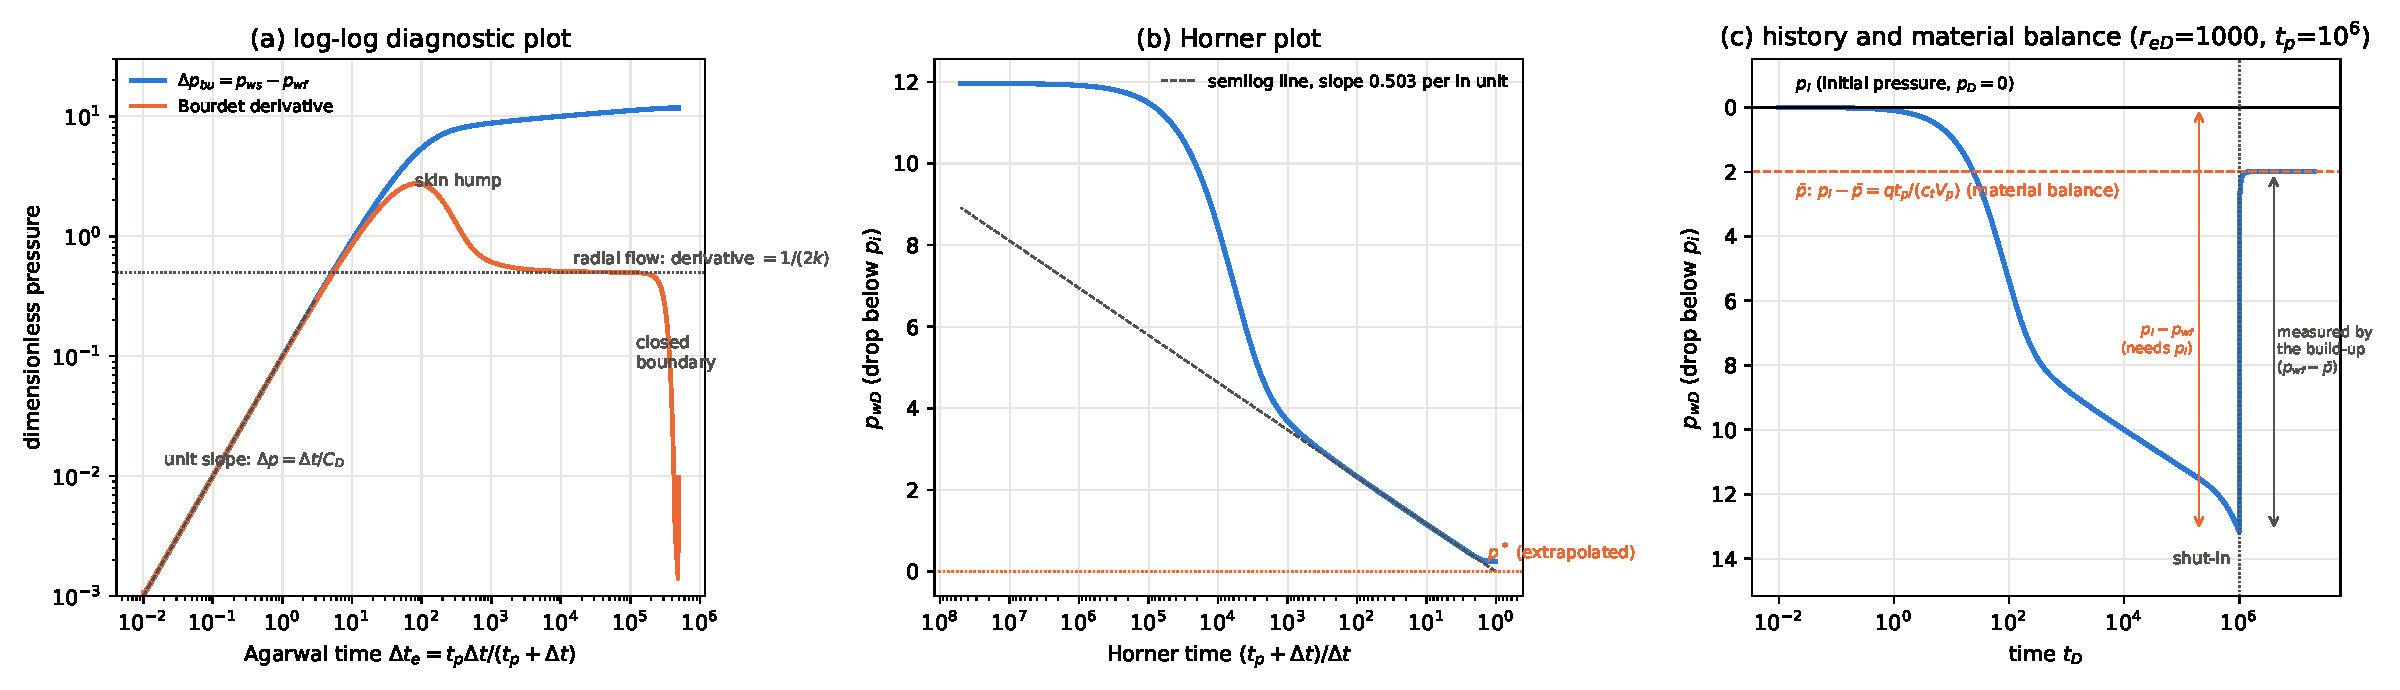
\includegraphics[width=\linewidth]{fig_theory.pdf}
  \caption{Build-up theory in a homogeneous closed reservoir ($k_D=1$, $C_D=10$, $S=5$), from the simulator.
  (a) Diagnostic plot for $\reD=2000$, $t_p = 5\times10^5$ (infinite-acting at shut-in): unit-slope storage, skin
  hump, radial-flow plateau at $1/2$, closed-boundary drop. (b) Horner plot of the same test: semilog slope
  $0.503$, extrapolated $p^* = p_i$. (c) Complete history of a longer-producing test ($\reD=1000$, $t_p=10^6$):
  the build-up stabilizes at the average pressure $\pb$ given by material balance; the gauge measures only the
  rise $p_{ws} - p_{wf}$, whereas $p_i - p_{wf}$ and $p_i - \pb$ require the initial pressure.}
  \label{fig:theory}
\end{figure}

If production lasted long enough for the boundary to be felt before shut-in, $p_{dd}(t_p+\Delta t)$ is no longer
semilog, the Horner line is distorted and $p^* \ne p_i$; the Matthews--Brons--Hazebroek (MBH) method relates
$p^* - \pb$ to the dimensionless production time $t_{pDA} = k t_p/(\phi\mu c_t A)$ of the drainage area $A$.

\subsection{Material balance and the role of the initial pressure}
\label{sec:mb}

In a closed reservoir, every barrel produced comes from the expansion of the fluid and rock in the drainage volume
and from the wellbore. After a production period $t_p$ at rate $q$ and a shut-in long enough for the pressure to
equalize at $\pb$,
\begin{equation}
  q B\, t_p = c_t V_p\,(p_i - \pb) + C\,(p_i - \pb), \qquad V_p = \pi\phi h\,(r_e^2 - r_w^2),
\end{equation}
which in the variables \eqref{eq:dimless} reads
\begin{equation}
  \pb_D = \frac{t_{pD}}{(\reD^2-1)/2 + C_D} .
  \label{eq:mb}
\end{equation}
This is independent of the permeability: the \emph{volume} of the reservoir, and hence $\reD$, follows directly
from the depletion $p_i - \pb$ and the produced volume. The test simulator satisfies \eqref{eq:mb} to rounding
error, and on stabilized synthetic build-ups it returns $\reD$ to $3\times10^{-7}$ (Section~\ref{sec:labels}).

The catch is what the gauge measures (Figure~\ref{fig:theory}c). A build-up records $p_{ws}(\Delta t)$, and its
interpretation uses the \emph{rise} $p_{ws} - p_{wf}$. Material balance needs the \emph{depletion}
$p_i - \pb = (p_i - p_{wf}) - (\pb - p_{wf})$: the build-up supplies the second term, but the first term needs
$p_i$. Three situations follow.

\begin{itemize}
  \item \textbf{$p_i$ known.} Typical for a new or exploration well: the initial pressure is measured by a
  formation tester, a drill-stem test or a static survey before production. Then $p_i - p_{wf}$ is known and the
  stabilized build-up gives $\reD$ by \eqref{eq:mb}. Even before stabilization, the apparent size
  $r_{\rm app}(\Delta t) = \sqrt{2 t_p/(p_{wf}-\Delta p_{bu}(\Delta t)) + 1}$ is a lower bound that converges to
  $\reD$; the neural model of Section~\ref{sec:nn} uses it as an input.
  \item \textbf{$p_i$ unknown, single build-up.} Only differences within the build-up are available. The boundary
  still shows up through its \emph{timing}, $t_D \approx \reD^2/(4k_D)$, but timing constrains
  $\reD^2/k$, not $\reD$: a larger reservoir with more permeable far field looks the same. The boundary distance is
  then only as good as the knowledge of the far-field permeability, which the build-up constrains least. This is
  the same ambiguity that makes the MBH method require $k$ and the shape of the drainage area.
  \item \textbf{$p_i$ unknown, more data.} Volume can still be measured without $p_i$ from pressure
  \emph{changes over produced volume}: the slope of the flowing pressure in pseudo-steady state
  (\eqref{eq:pss}, a reservoir limit test), or the difference between the stabilized pressures of two build-ups
  separated by a known production (the two flow periods of a drill-stem test).
\end{itemize}
The average pressure $\pb$ itself is usually an \emph{output} of the build-up (via $p^*$ and MBH), not an input.

\subsection{Heterogeneous reservoirs: what the derivative measures}
\label{sec:hetero}

When $k$ varies with radius, there is no single radial-flow plateau. At time $t$ the derivative reflects the
permeability around the radius of investigation $2\sqrt{k t}$, averaged over a region of roughly half a decade in
radius. Radial resistances add in series, so the natural average of $k$ over a ring $[a, b]$ is the
\emph{log-harmonic mean}
\begin{equation}
  \bar k_{[a,b]} = \ln\frac{b}{a} \bigg/ \int_a^b \frac{\dd r}{r\,k(r)} ,
  \label{eq:ringmean}
\end{equation}
and any near-well region of different permeability acts as a skin relative to whatever $k$ is read farther out.
A build-up therefore constrains a smoothed radial permeability \emph{profile}, sharply near the well and more
loosely farther out; a single pair $(k, S)$ is a summary whose value depends on the time window chosen.
Section~\ref{sec:labels} quantifies this on the synthetic data.

%======================================================================
\section{Synthetic build-up data}
\label{sec:data}

\subsection{Simulator}
\label{sec:solver}

Equation \eqref{eq:diffD} is solved by vertex-centered finite volumes on a log-spaced grid
$r_{D,j} = e^{jD}$, $D = \ln 1000/1023 \approx 0.0068$ (about 850--1190 nodes for $\reD = 300$--$3000$). Face
fluxes $k_{j+1/2}(p_{j+1}-p_j)/D$ are exact for steady radial flow; $k_{j+1/2}$ is the harmonic mean of the node
values, exact for a permeability jump at the face. The unknowns $(p_{wD}, p_0, \dots, p_{N-1})$ keep the system
tridiagonal, including storage \eqref{eq:storage} and thin skin; time integration is variable-step BDF2, restarted
at rate changes. A full run from $t_D = 0$ to $10^7$ takes about 0.05\,s. Table~\ref{tab:solver} summarizes the
validation.

\begin{table}[h]
  \centering
  \small
  \begin{tabular}{@{}p{0.66\linewidth}p{0.28\linewidth}@{}}
    \toprule
    Check ($k_D = 1$ unless stated) & Result \\
    \midrule
    van Everdingen--Hurst (Laplace, Stehfest), $\reD=300$, $t_D = 0.1$--$10^7$, $C_D\in\{0,100\}$, $S\in\{0,5\}$ & $\le 3\times10^{-4}$ relative \\
    line source, $t_D = 10^3$--$10^5$ & $<10^{-3}$ \\
    pseudo-steady state \eqref{eq:pss} & $<10^{-4}$ \\
    storage unit slope, $C_D = 10^3$ & $<2\times10^{-3}$ \\
    mass balance, heterogeneous $k$, shut-in & exact to $10^{-9}$ \\
    simulated shut-in vs superposition \eqref{eq:superposition}, heterogeneous $k$ & $<10^{-3}$ of the build-up change \\
    radial-flow interpretation (plateau $k$, semilog $S$), with storage and skin & $k$ within 1.5\,\%, $S$ within 0.15 \\
    \bottomrule
  \end{tabular}
  \caption{Validation of the simulator and the build-up tools.}
  \label{tab:solver}
\end{table}

Because of superposition, one unit-rate drawdown per reservoir, stored at 200 log-spaced times in $[10^{-2},
10^7]$, generates every build-up; between the stored times the drawdown is interpolated by a cubic spline in
$\ln t$ (accuracy $3\times10^{-6}$).

A unit convention: the solver's thin skin is scaled with $k_{\rm ref}$, whereas the skin read from a build-up is
relative to the formation permeability, $S_{\rm wt} = k_D S$.

\subsection{Permeability model}

Each reservoir has
\begin{equation}
  \ln k_D(r) = m + g(\ln r) + \delta\,\mathbf 1[r < r_s], \qquad \text{clipped to } [-3, 3],
\end{equation}
with a mean shift $m\sim N(0, 0.3^2)$, a zero-mean Gaussian random field $g$ in $\ln r$ with squared-exponential
covariance of standard deviation $\sigma\sim U(0.5,1)$ and correlation length $\ell\sim U(0.3,1.5)$, and, in half
of the reservoirs, a skin zone of radius $r_s\sim\log U[2,20]$ and log permeability ratio
$\delta = \ln(k_s/k)\sim U(\ln 0.1, \ln 5)$. The field is sampled by circulant embedding (FFT) on the uniform
$\ln r$ grid. It is stationary in $\ln r$: its statistics are the same per unit of $\ln r$ from the wellbore
outward (measured spread 0.82--0.85 at every radius), so features are larger farther from the well
(Figure~\ref{fig:logk}).

\begin{figure}[h]
  \centering
  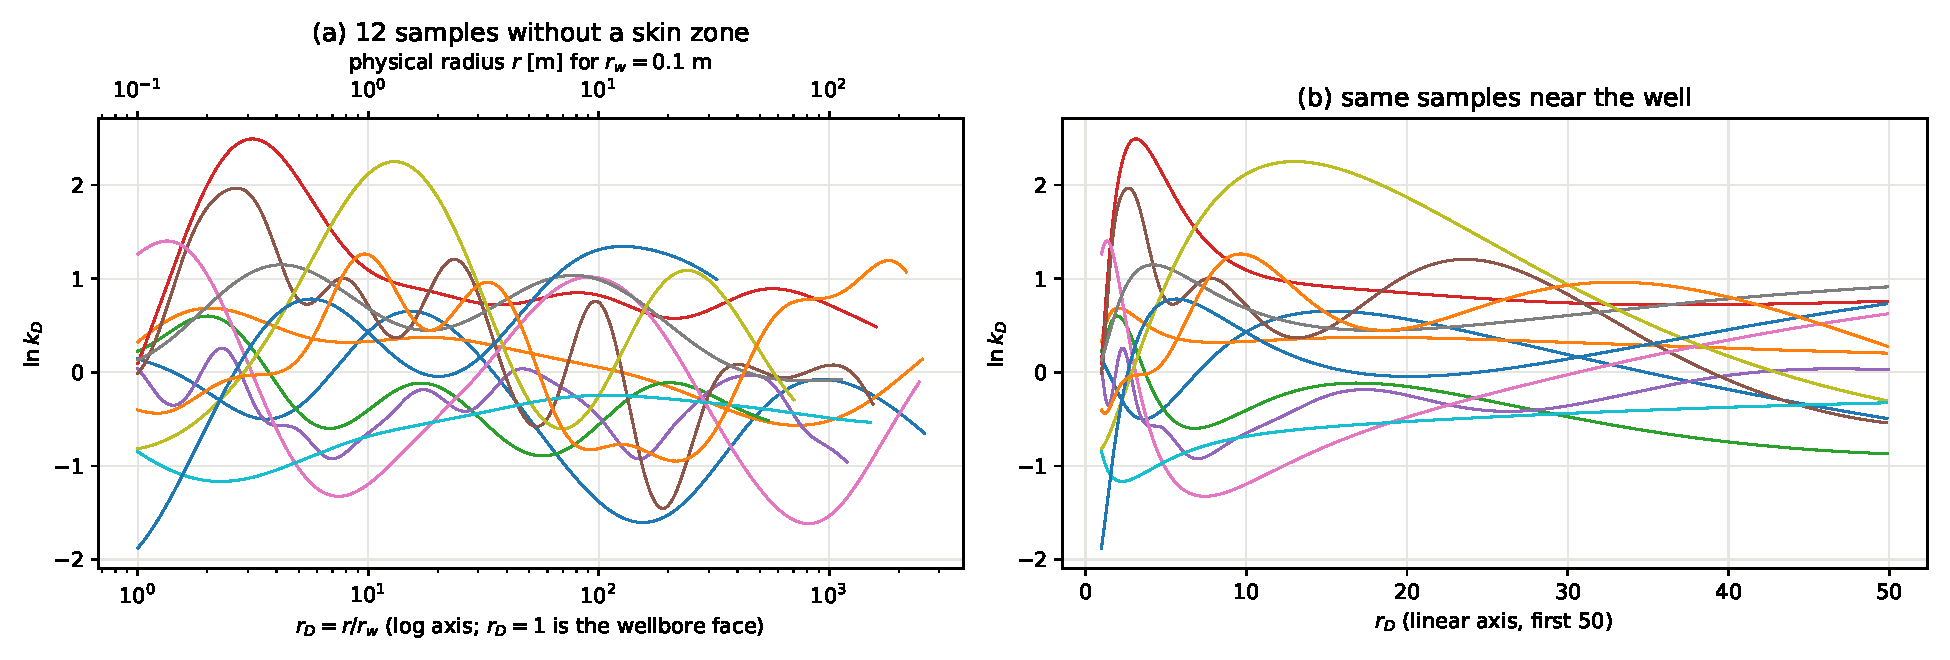
\includegraphics[width=0.95\linewidth]{fig_logk_samples.pdf}
  \caption{Twelve permeability fields without a skin zone. (a) Log radius, with the physical radius for
  $r_w=0.1$\,m on top: variation starts at the wellbore face. (b) Linear radius near the well: stationarity in
  $\ln r$ packs the variation close to the well.}
  \label{fig:logk}
\end{figure}

\subsection{Dataset}

The dataset has 20\,000 reservoirs (18\,000 training, 1\,000 validation, 1\,000 test), generated in six minutes on
eight cores. Per reservoir: $\reD\sim\log U[300,3000]$; $C_D = 0$ in 20\,\% of the reservoirs and
$\log U[0.1, 10^3]$ otherwise; the permeability field above; one unit-rate drawdown (stored in float64, since
build-ups are small differences of drawdown values). In the training split the radial-flow permeability ranges
from 0.07 to 7.2 (median 0.84), and the boundary is felt within $\Delta t_D = 9\times10^6$ in 99.9\,\% of the
reservoirs. Figure~\ref{fig:examples} shows four test reservoirs.

\begin{figure}[h]
  \centering
  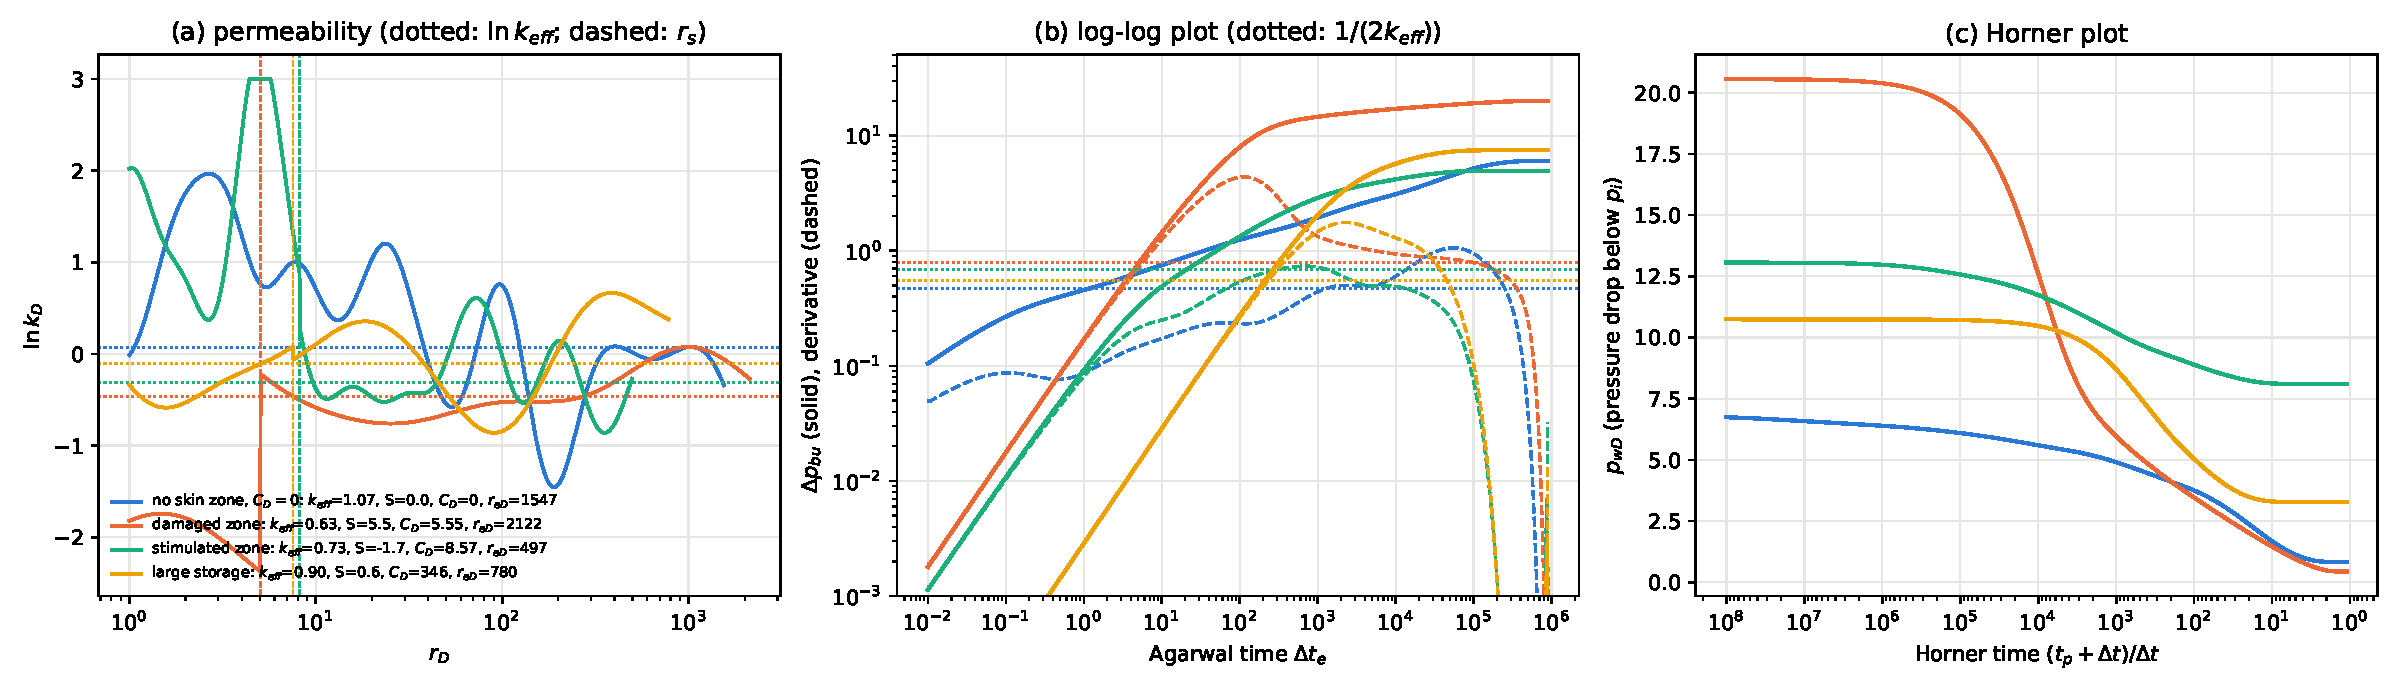
\includegraphics[width=\linewidth]{fig_examples.pdf}
  \caption{Four test reservoirs after $t_p=10^6$. (a) $\ln k_D$ (dotted: the whole-reservoir average; dashed:
  $r_s$). (b) Diagnostic plot: pressure change (solid) and derivative (dashed); the dotted levels are where the
  derivative would sit if a single permeability applied. (c) Horner plot. The derivative of the heterogeneous
  reservoirs wanders instead of forming one plateau.}
  \label{fig:examples}
\end{figure}

%======================================================================
\section{What a build-up actually measures}
\label{sec:labels}

Before training anything, the natural labels were checked against a classical interpretation of each test build-up
($t_p = 10^6$, radial-flow window chosen with the true parameters: after storage, before the boundary;
684 of 1000 test reservoirs have such a window). Figure~\ref{fig:labels} and Table~\ref{tab:labels} summarize.

\begin{table}[h]
  \centering
  \small
  \begin{tabular}{@{}p{0.3\linewidth}p{0.4\linewidth}p{0.24\linewidth}@{}}
    \toprule
    Label & Check & Result \\
    \midrule
    $\reD$ & material balance \eqref{eq:mb} from the stabilized build-up (695 tests) & exact to $3\times10^{-7}$ \\
    $k$ (whole-reservoir log-harmonic mean) & vs derivative plateau & median error 23\,\%, 90th pct.\ ${\sim}2\times$ \\
    $k$ over the investigated ring & vs derivative plateau & median error 18\,\% \\
    $S$ (relative to the whole-reservoir $k$) & vs semilog skin & median difference 1.1, 90th pct.\ 6 \\
    \bottomrule
  \end{tabular}
  \caption{Label check on the test split.}
  \label{tab:labels}
\end{table}

\begin{figure}[h]
  \centering
  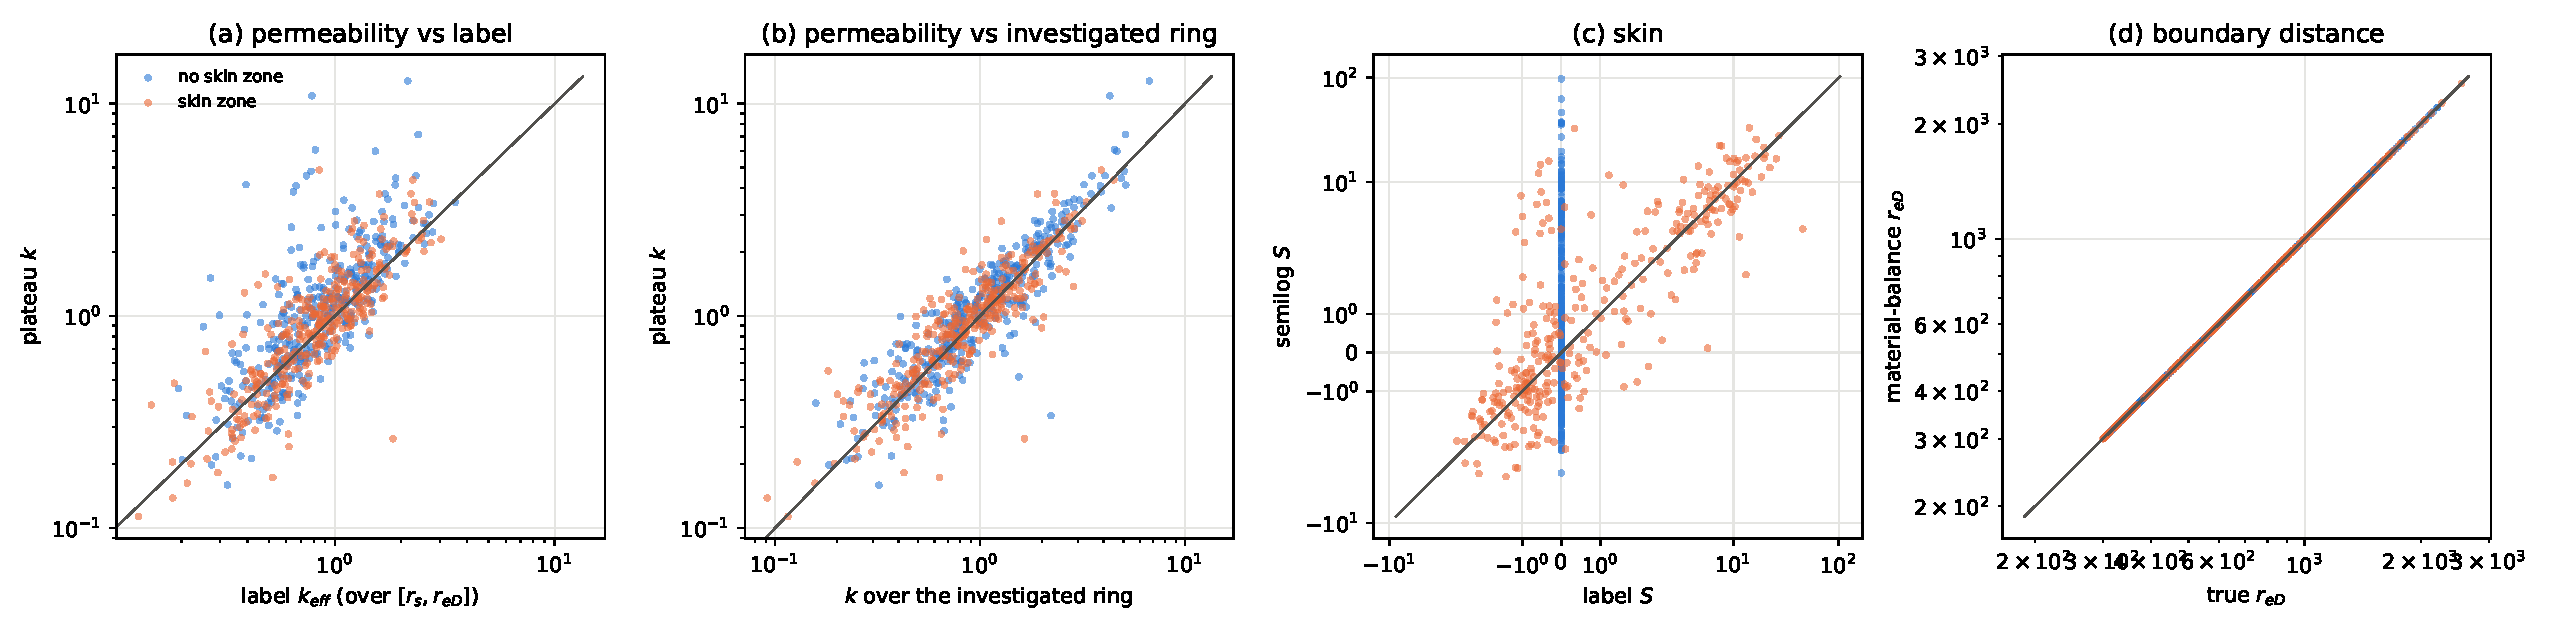
\includegraphics[width=\linewidth]{fig_label_check.pdf}
  \caption{Classical interpretation vs labels. (a, b) The plateau permeability agrees better with the ring actually
  investigated than with the whole-reservoir average. (c) Reservoirs without a skin zone (label $S=0$) read
  semilog skins from $-1$ to about 100: near-well heterogeneity acts as skin. (d) Material balance recovers
  $\reD$ exactly.}
  \label{fig:labels}
\end{figure}

The boundary distance is a clean label; a single $(k, S)$ pair is not, as anticipated in
Section~\ref{sec:hetero}. The inverse problem was therefore posed with the targets
\begin{itemize}
  \item $\ln \bar k$ by \eqref{eq:ringmean} over eight rings in $r_D$: $[1,2]$, $[2,5]$, $[5,10]$, $[10,30]$,
  $[30,100]$, $[100,300]$, $[300,1000]$, $[1000,3000]$, each clipped at $\reD$ and masked when less than a radius ratio 1.5 of it lies inside;
  \item $\ln C_D$, with a separate no-storage flag;
  \item $\ln\reD$.
\end{itemize}
Any skin definition can be computed from the profile afterwards.

%======================================================================
\section{Model-based inversion}
\label{sec:inversion}

The most direct inverse method fits the simulator to the data. The unknowns are $\ln k$ at 16 control points
(linear in $\ln r$ between $r_D = 1$ and 3000), $\ln C_D$ and $\ln\reD$; the misfit is the relative error of the
build-up change and of the drawdown at shut-in $p_i - p_{wf}$, for 1\,\% gauge noise, plus a smoothness penalty and
a weak prior on $\ln k$; the minimization is Levenberg--Marquardt-type least squares started from the classical
estimates, and the uncertainty is the Gauss--Newton covariance. On test reservoir 486 (damaged zone on a
low-permeability near-well region, $S = 9.2$) it recovers $C_D = 0.582$ (true 0.584), $\reD = 1658\pm10\,\%$
(true 1645), and the ring permeabilities to within 0.04 in $\ln k$ for $r_D<100$ and about 0.25 beyond
(Figure~\ref{fig:invert}), in 10--40\,s. Fitting the build-up change alone, without $p_i - p_{wf}$, let $\reD$
drift to 1246: the material-balance information enters only through $p_i$.

\begin{figure}[h]
  \centering
  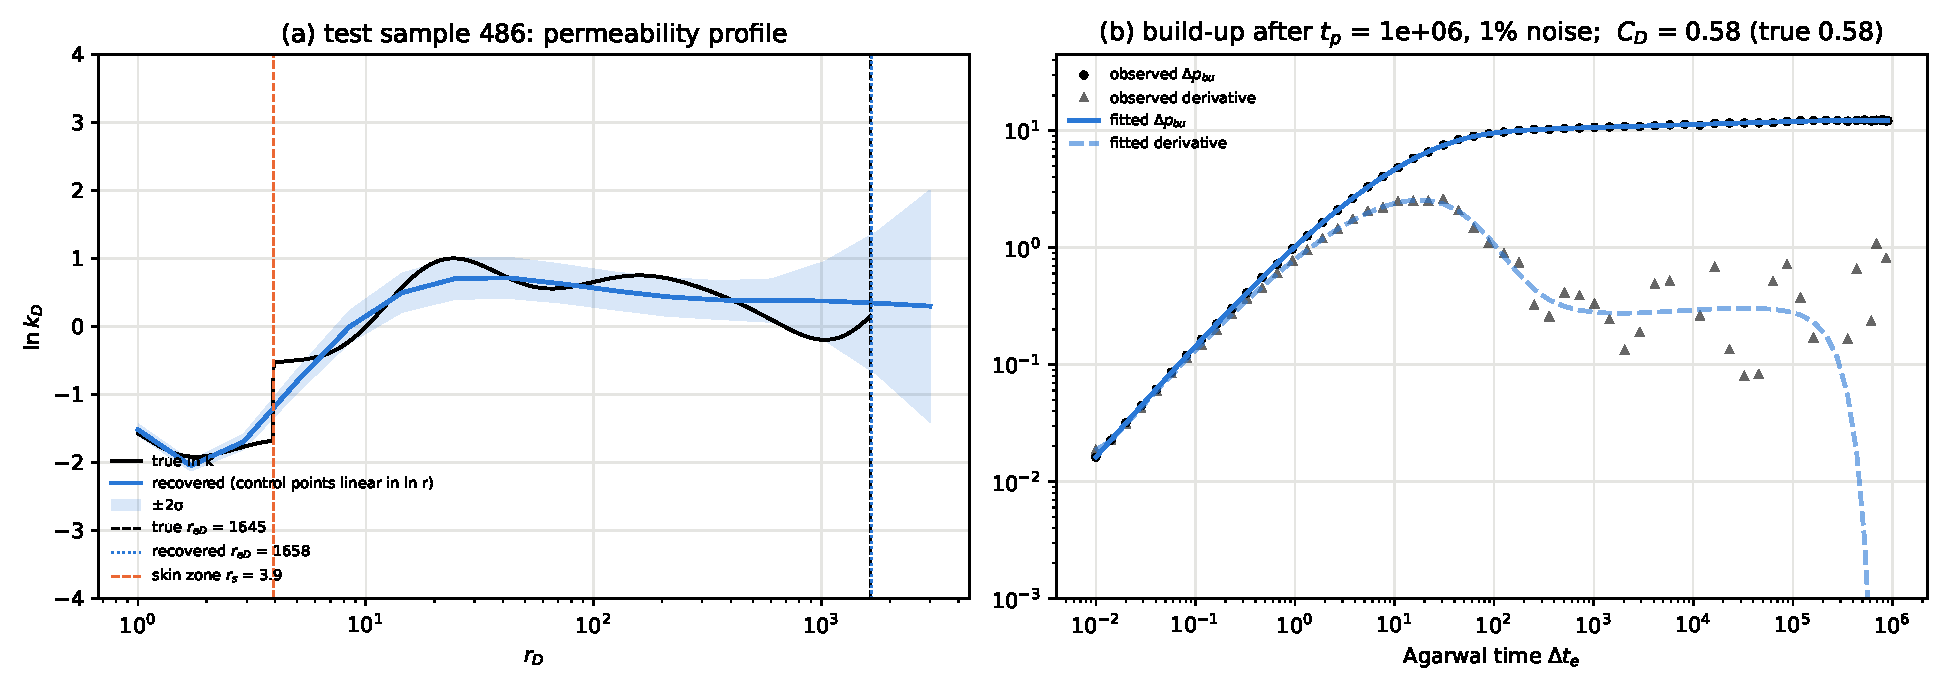
\includegraphics[width=\linewidth]{fig_invert_486.pdf}
  \caption{Model-based inversion of test reservoir 486 with 1\,\% noise. (a) True and recovered $\ln k$ with
  $\pm2\sigma$; the skin step is smoothed over one control spacing. (b) Observed and fitted build-up.}
  \label{fig:invert}
\end{figure}

%======================================================================
\section{A neural inverse model}
\label{sec:nn}

The model-based inversion is accurate but takes tens of seconds and needs a starting point. A neural network can
learn the same map from data once and then evaluate it in milliseconds.

\subsection{Inputs, targets and realism}

Every training step forms fresh build-ups from the stored drawdowns by superposition, on a fixed grid of 128
log-spaced shut-in times in $[10^{-2}, 9\times10^6]$. The input channels are: $\ln\Delta p_{bu}$; the log-derivative
$\dd\ln\Delta p_{bu}/\dd\ln\Delta t$; the time coordinate; $\ln t_p$; $\ln(p_i - p_{wf})$ and a $p_i$-known flag;
a validity mask; the apparent material-balance radius $r_{\rm app}(\Delta t)$ (Section~\ref{sec:mb}); and the
gauge noise level. Realism: $t_p\sim\log U[10^4,10^6]$; relative gauge noise $\log U[10^{-4},10^{-2}]$;
$p_i$ unknown in 25\,\% of the examples; half of the tests truncated at $\Delta t_{\max}\sim\log U[10^6, 9\times10^6]$
(days of shut-in). Production and test length are drawn independently of the reservoir: a test length tied to
$\reD^2/k$ would let the model read $\reD$ from the length of the record.

\subsection{Architecture and loss}

A Fourier neural operator along $\ln\Delta t$ (lift, four spectral layers with 24 modes and width 48, pointwise
paths, GELU) extracts features at all time scales; masked mean and max pooling over the valid part of the test
feed an MLP that outputs a mean and a log-variance for each of the ten targets and a logit for the no-storage flag
(0.48 M parameters). The loss is the $\beta$-weighted Gaussian negative log-likelihood ($\beta=0.5$): with the plain
likelihood the gradient of a target's mean scales with its inverse predicted variance, and $\reD$, initially
assigned a large variance, was never learned (Table~\ref{tab:runs}, first row).

\subsection{Development}

Table~\ref{tab:runs} traces the changes that mattered.

\begin{table}[h]
  \centering
  \small
  \begin{tabular}{@{}p{0.08\linewidth}p{0.32\linewidth}p{0.3\linewidth}p{0.22\linewidth}@{}}
    \toprule
    Run & Change & $\reD$ median error: all / $p_i$ known / $p_i$ unknown & Test set \\
    \midrule
    base & Gaussian NLL & not learned (prior spread) & short tests \\
    beta & $\beta$-NLL & 35 / 34 / 39\,\% & short tests \\
    mb & + material-balance input $r_{\rm app}$ & 31 / 27 / 41\,\% & short tests \\
    long & realistic production and test lengths & 13.6 / 9.5 / 28.5\,\% & realistic, 1\,\% noise \\
    noise & noise level randomized and given as input & 14.1 / 10.1 / 29.6\,\% & realistic, 1\,\% noise \\
         &  & 3.4 / 2.0 / 20.0\,\% & realistic, 0.1\,\% noise \\
         &  & 1.7 / 1.1 / 19.6\,\% & realistic, 0.01\,\% noise \\
    \bottomrule
  \end{tabular}
  \caption{Development of the inverse model (1000 test reservoirs, four build-ups each). ``Short tests'': production
  from $t_p = 10^3$ and truncation down to $\Delta t = 10^2$, where the boundary is often never felt.}
  \label{tab:runs}
\end{table}

Three lessons stand out. First, the material-balance input made the model use $p_i$: before it, knowing $p_i$ barely
helped, and on stabilized tests the model was worse than the material-balance formula. Second, most of the
improvement from ``mb'' to ``long'' came from the test data, not from training: evaluated on the realistic tests,
the ``mb'' model already reaches 13.8\,\% ($p_i$ known 9.9\,\%). Tests that are too short do not contain $\reD$.
Third, a model trained at 1\,\% noise does not exploit a precise gauge; told the noise level, it does.

\subsection{Results}

Figure~\ref{fig:eval} shows the final model on the test set at 0.1\,\% noise, Figure~\ref{fig:noise} its dependence
on gauge precision, and Table~\ref{tab:final} the numbers.

\begin{table}[h]
  \centering
  \small
  \begin{tabular}{@{}p{0.46\linewidth}ccc@{}}
    \toprule
    Gauge noise & 0.01\,\% & 0.1\,\% & 1\,\% \\
    \midrule
    $\reD$ median error, $p_i$ known & 1.1\,\% & 2.0\,\% & 10\,\% \\
    \quad 90th percentile & 5.9\,\% & 16\,\% & 47\,\% \\
    $\reD$ median error, $p_i$ unknown & 20\,\% & 20\,\% & 30\,\% \\
    \quad 90th percentile & 51\,\% & 51\,\% & 73\,\% \\
    $\ln C_D$ mean absolute error & 0.026 & 0.023 & 0.042 \\
    ring $\ln k$ MAE, $r_D < 100$ & 0.04--0.09 & 0.04--0.09 & 0.08--0.16 \\
    ring $\ln k$ MAE, $r_D$ 100--300 & 0.06 & 0.06 & 0.14 \\
    ring $\ln k$ MAE, $r_D$ 300--1000 & 0.15 & 0.17 & 0.33 \\
    ring $\ln k$ MAE, $r_D$ 1000--3000 & 0.27 & 0.34 & 0.50 \\
    no-storage flag accuracy & 100\,\% & 100\,\% & 100\,\% \\
    coverage of $\pm2\sigma$: rings / $C_D$ / $\reD$ & 94 / 92 / 96\,\% & 96 / 97 / 97\,\% & 90 / 92 / 94\,\% \\
    classical material balance: usable in & 75\,\% & 63\,\% & 9\,\% \\
    \quad its median $\reD$ error & 0.15\,\% & 1.3\,\% & 8.0\,\% \\
    \quad model on the same tests & 1.1\,\% & 1.9\,\% & 7.6\,\% \\
    \bottomrule
  \end{tabular}
  \caption{Final (noise-aware) model on the test set. ``Usable'' classical material balance: $p_i$ known and the
  build-up stabilized.}
  \label{tab:final}
\end{table}

\begin{figure}[h]
  \centering
  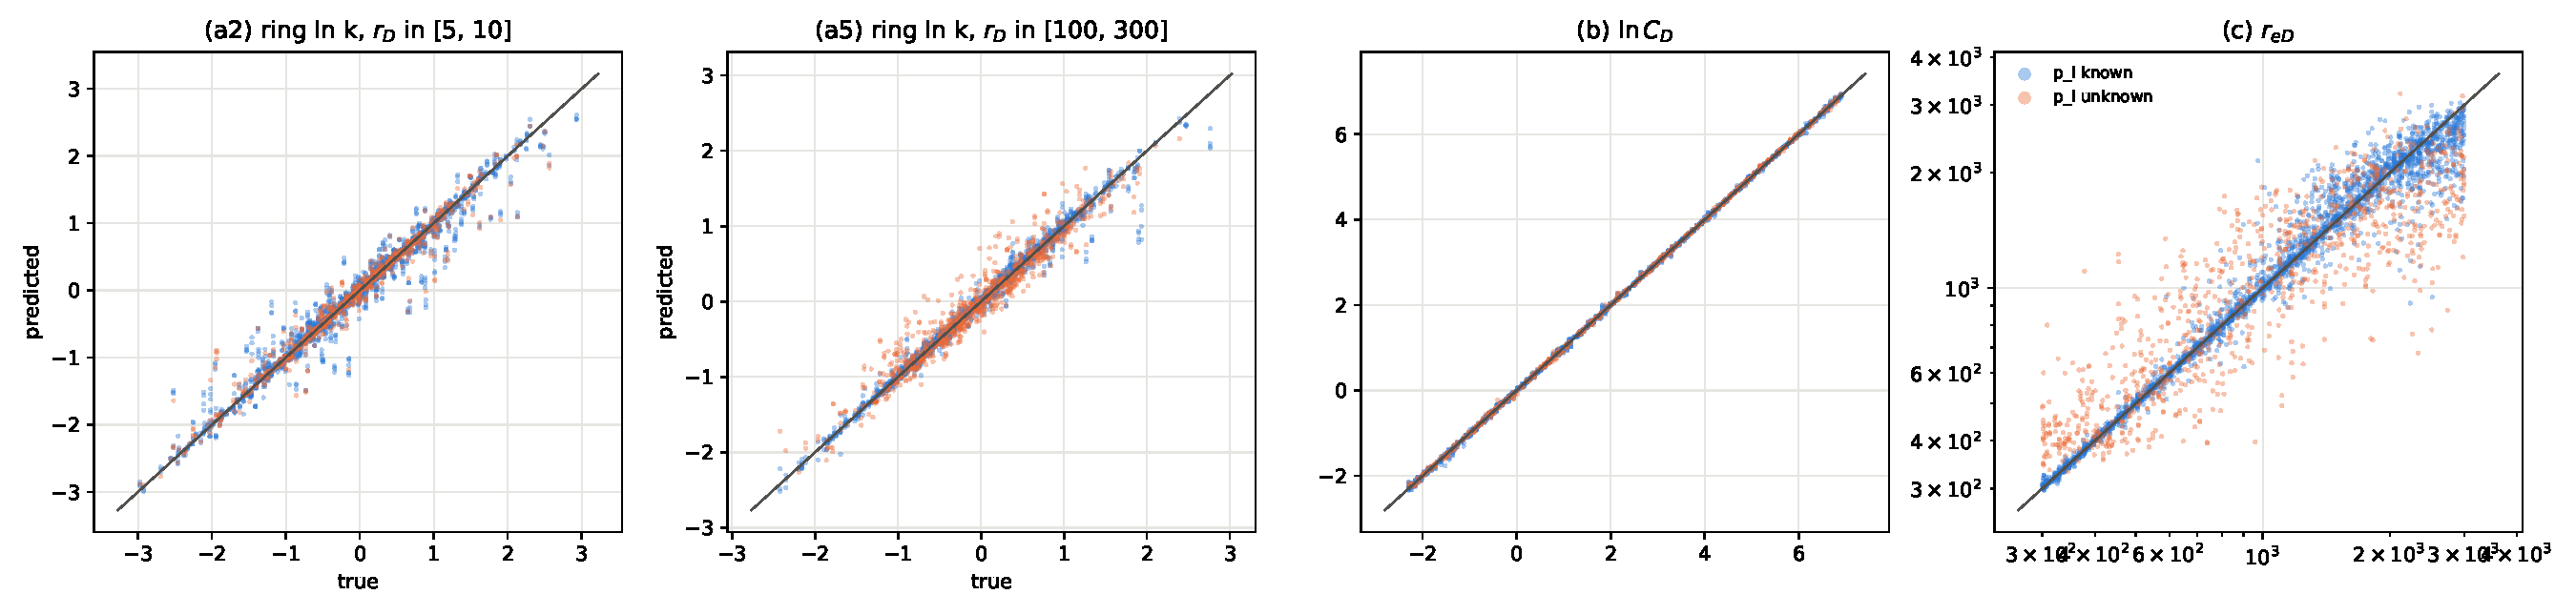
\includegraphics[width=\linewidth]{fig_inverse_eval_noise_model.pdf}
  \caption{Final model on the test set at 0.1\,\% gauge noise: predicted vs true ring permeabilities near
  ($r_D$ 5--10) and far (100--300) from the well, $\ln C_D$, and $\reD$ (blue: $p_i$ known).}
  \label{fig:eval}
\end{figure}

\begin{figure}[h]
  \centering
  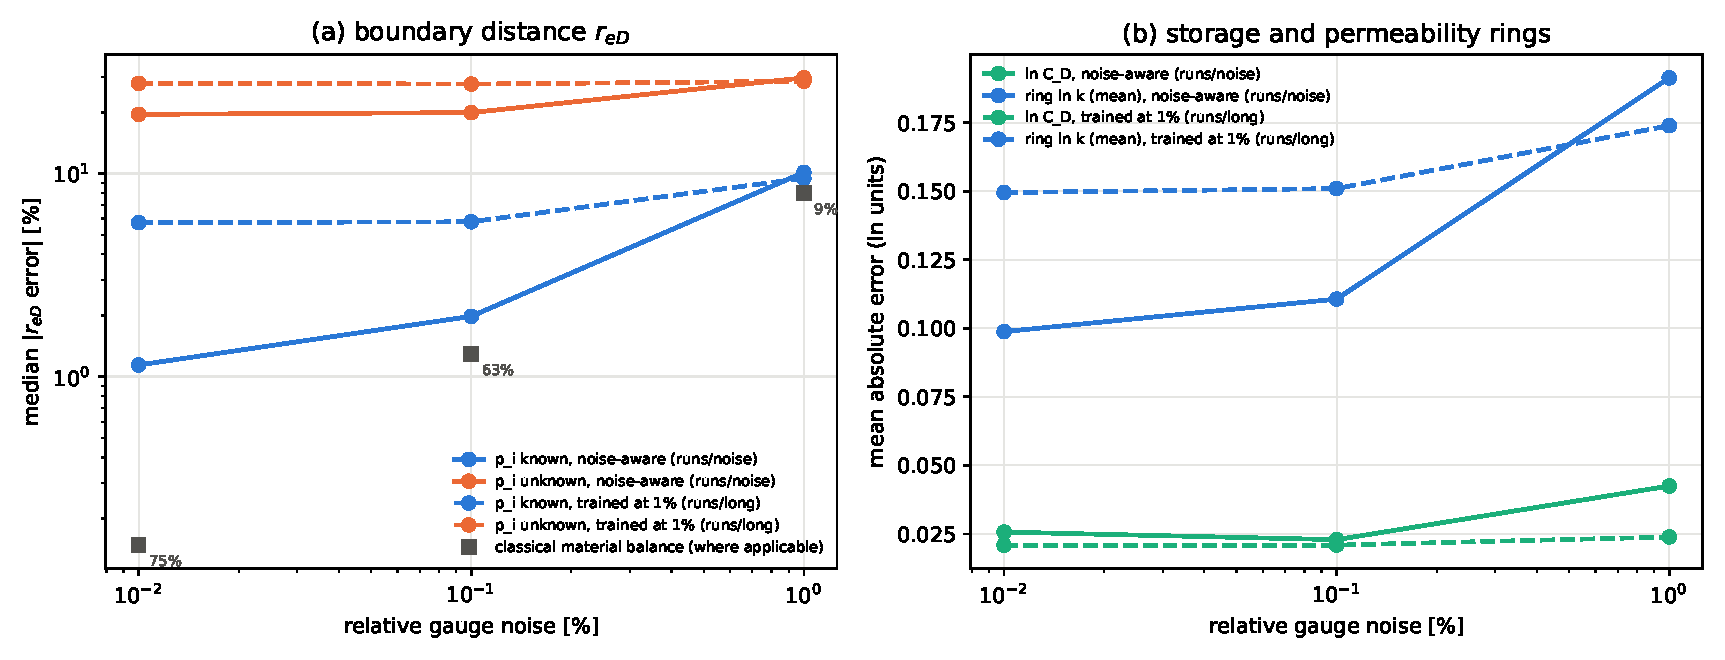
\includegraphics[width=0.95\linewidth]{fig_noise_summary.pdf}
  \caption{Dependence on the gauge noise. (a) $\reD$ error with and without $p_i$ for the noise-aware model (solid)
  and a model trained at 1\,\% noise (dashed), and classical material balance where it applies (percentages: share
  of tests where it is usable). (b) Storage and ring errors.}
  \label{fig:noise}
\end{figure}

\paragraph{Uncertainty.} The predicted standard deviations are calibrated: the empirical coverage follows the nominal
level at every level (Figure~\ref{fig:calibration}, model trained at 1\,\% noise), so no post-hoc scaling is used. The
noise-aware model is slightly overconfident at 1\,\% noise (90--94\,\% coverage of $\pm2\sigma$).

\begin{figure}[h]
  \centering
  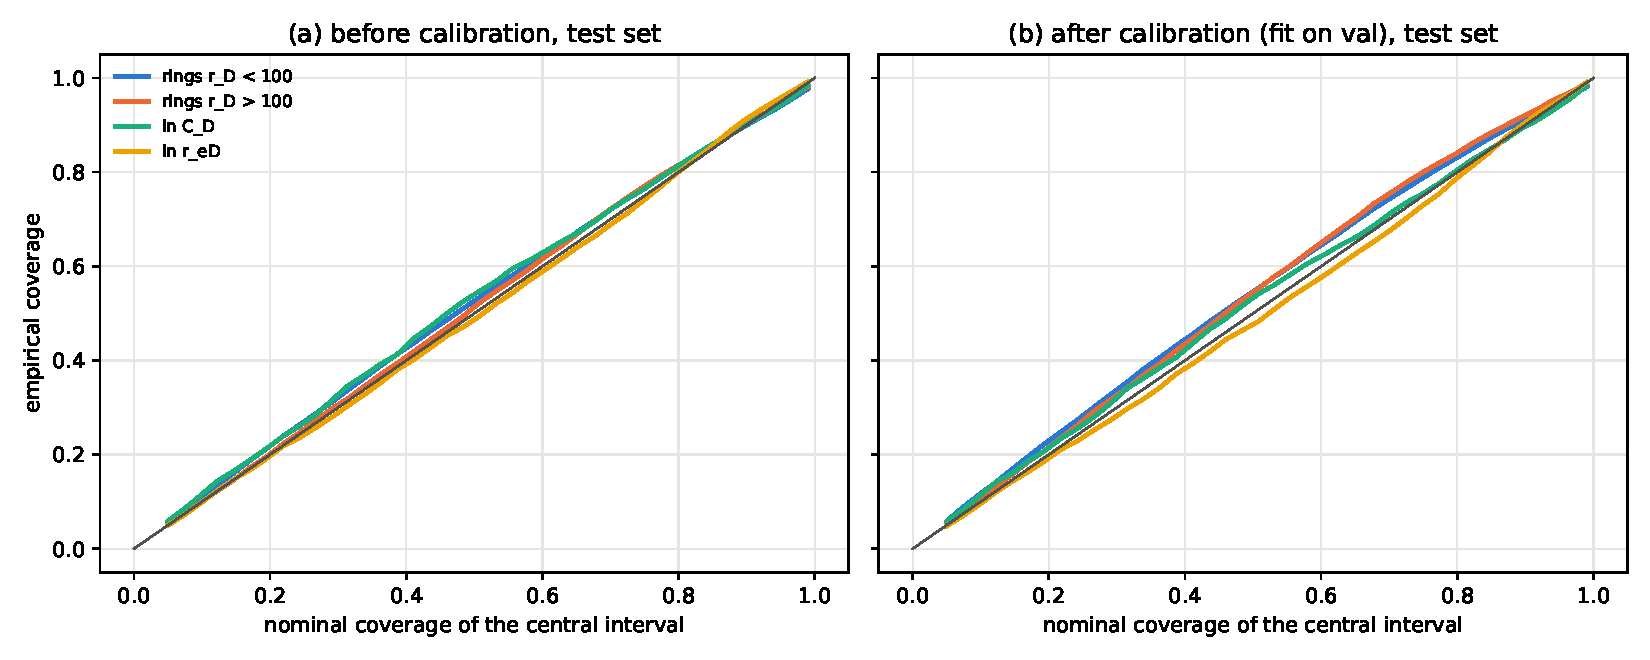
\includegraphics[width=0.8\linewidth]{fig_calibration.pdf}
  \caption{Reliability of the predicted uncertainties on the test set (model trained at 1\,\% noise): empirical vs
  nominal coverage of central intervals, before and after a validation-fitted scaling. The raw uncertainties are
  already calibrated.}
  \label{fig:calibration}
\end{figure}

\subsection{When the boundary distance is not determined}

The largest $\reD$ errors (the worst 10\,\%) have two causes (Figure~\ref{fig:tail}, 1\,\% noise).
The first is \emph{drainage before shut-in}, $t_p k/\reD^2$: with $p_i$ known the median error is 33\,\% when it is
below 0.01 and 6.9\,\% above (3.7\,\% at 0.1\,\% noise). With little production the depletion
$p_i - \pb \approx 2t_p/\reD^2$ is buried in the gauge noise, however long the shut-in. The second is a missing
$p_i$ (Section~\ref{sec:mb}). The test length matters little once shut-ins last days. The model recognizes these
cases: its predicted standard deviation of $\ln\reD$ doubles (0.47 against 0.24) and 82\,\% of these errors
remain within $\pm2\sigma$. A practical design rule follows: to determine the boundary distance to within about
7\,\% at 1\,\% gauge noise with $p_i$ known, produce for $t_p \gtrsim 0.01\,\reD^2/k$ in dimensionless time
before the shut-in.

\begin{figure}[h]
  \centering
  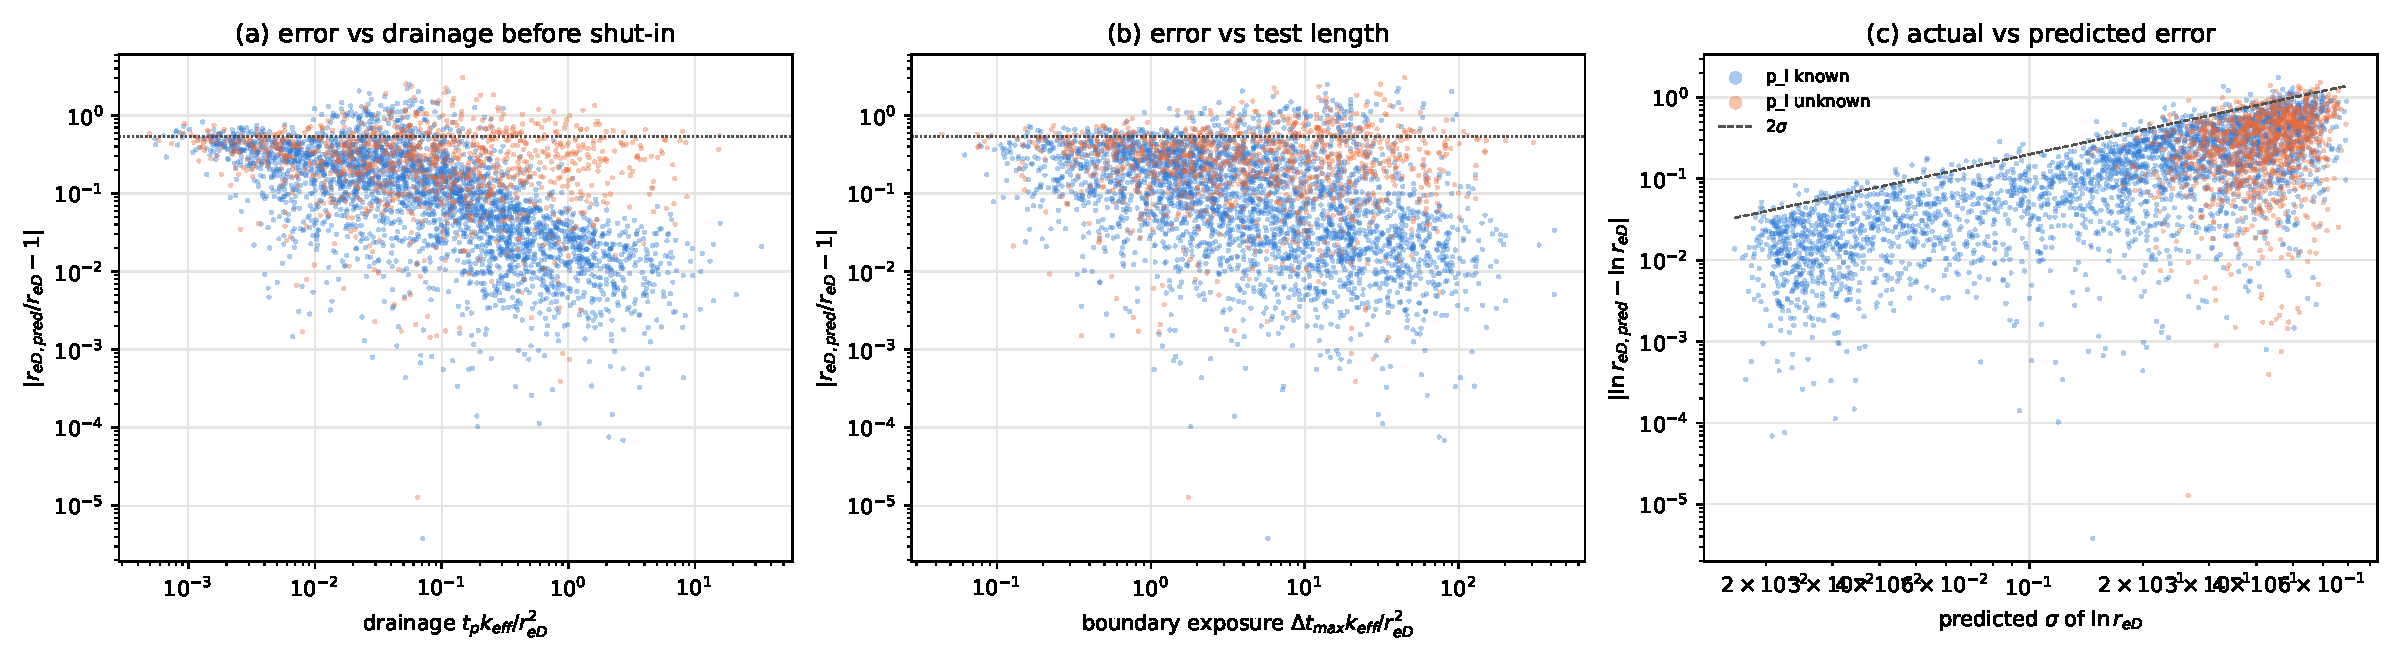
\includegraphics[width=\linewidth]{fig_re_tail.pdf}
  \caption{$\reD$ error at 1\,\% noise vs (a) drainage before shut-in, (b) boundary exposure during the test, and
  (c) the predicted uncertainty (dashed: $2\sigma$).}
  \label{fig:tail}
\end{figure}

%======================================================================
\section{Discussion}

\paragraph{Compared with classical interpretation.} In heterogeneous reservoirs the classical plateau permeability
depended on the chosen window (median error 23\,\%) and the semilog skin was misleading; the model returns a radial
permeability profile instead. It gives an estimate for every test, including those where the classical specialized
methods do not apply (at 1\,\% noise, classical material balance was usable in 9\,\% of the tests), it estimates
all parameters jointly with calibrated uncertainties ($C_D$ to 2--4\,\% against about 9\,\% from the classical unit slope), and it
takes milliseconds per test. Where an exact formula applies it remains better: on stabilized tests with a precise
gauge and known $p_i$, material balance gives $\reD$ to 0.15\,\% against 1.1\,\% for the model.

\paragraph{Limitations.} The model is only valid within the physics it was trained on: one well, a closed circular
boundary, radial heterogeneity, one constant-rate flow period, single-phase flow. Faults, channels, dual porosity,
multiphase effects and rate histories are outside its training, and its uncertainty is not guaranteed to flag such
data. Like classical analysis it needs $q$, $B$, $\mu$, $h$, $\phi c_t$ and $r_w$ to make the data dimensionless. It
has not yet been tested on field data.

\paragraph{Without the initial pressure.} The remaining 20--30\,\% error in $\reD$ without $p_i$ is the
volume--permeability ambiguity of Section~\ref{sec:mb}. It can be reduced with more data rather than a better
network: the flowing-pressure record before shut-in (its pseudo-steady-state slope measures the pore volume without
$p_i$), or two build-ups separated by a known production.

\paragraph{Next steps.} Recover the accuracy at 1\,\% noise (longer or wider training); report classical material
balance where it applies; add the flowing period as an input; benchmark the network against the model-based
inversion on many tests; widen the training physics; test on field build-ups.

\appendix
\section{Reproducing the results}

All code is in \texttt{buildup/} (independent of the rest of the repository); tests:
\texttt{pytest buildup/tests} (52 tests). Main scripts: \texttt{solver.py}, \texttt{analytic.py} (reference
solutions), \texttt{wells.py} (build-up tools), \texttt{permeability.py}, \texttt{dataset.py},
\texttt{invert.py}, \texttt{examples.py}, \texttt{model.py}, \texttt{train.py}, \texttt{evaluate.py},
\texttt{calibrate.py}, \texttt{analyze\_re\_tail.py}; figures by the \texttt{fig\_*.py} scripts. The plan and the
full record of decisions and results are in \texttt{buildup/tasks.md}.

\end{document}
